\documentclass[12 pt]{exam}
\usepackage{graphicx, enumitem, amsmath, amssymb}
\graphicspath{ {./images/} }
\usepackage{tikz, pgfplots}
\pgfplotsset{compat=1.16}
\usetikzlibrary{shapes,arrows}
%\usepackage{Minion Pro}
\printanswers

\title{3.2: Market Competition and Surpluses - Practice Problems (Answers)}
\author{Ryan Safner}
\date{ECON 306 - Spring 2020}

\begin{document}

\maketitle

The supply and demand in the market for tomatoes are estimated to be:

$$\begin{aligned}
q_D&=1000-200p\\
q_S&=200p-200\\ \end{aligned}$$

\begin{questions}

\question Calculate the market-clearing price and quantity exchanged.

\begin{solution}
	\begin{align*}
	q_D&=q_S && \text{Definition of equilibrium}\\
	1000-200p&=200p-200 && \text{Plugging in demand and supply functions}\\
	1000&=400p-200 && \text{Adding } 200p \text{ to both sides}\\
	1200&=400p && \text{Adding } 200 \text{ to both sides}\\
	3&=p^* && \text{Dividing both sides by }400\\
	\end{align*}
	Now finding equilibrium quantity, q* using Demand: 
	\begin{align*}
	q_D&=1000-200p && \text{The demand function}\\
	q_D&=1000-200(3) && \text{Plugging in } p^*=3	\\
	q_D&=1000-600 && \text{Multiplying}\\
	q^*&=400 && \text{Subtracting}\\
	\end{align*}

\end{solution}

\question Find the inverse demand function and inverse supply function.

\begin{solution}

First, demand:

\begin{align*}
	q_D&=1000-200p && \text{The demand function}\\
	q_D+200p&=1000 && \text{Adding }200p \text{ to both sides}\\
	200p&=1000-q_D && \text{Subtracting }q_D \text{ from both sides}\\
p&=5-0.005q_D && \text{Dividing both sides by }200\\
\end{align*}
The demand choke price is \$5 and the slope is $-0.005$ (or $-\frac{1}{200}$).   \medskip \\
Then supply:
\begin{align*}
	q_S&=200p-200 && \text{The supply function}\\
q_S+200&=200p && \text{Adding 200 to both sides}\\
0.005q_S+1&=p && \text{Dividing both sides by 200}\\
\end{align*}
The supply choke price is \$1 and the slope is 0.005 (or $\frac{1}{200}$) \bigskip \\

\end{solution}

\question Sketch a graph of this market, labelling key points.

\begin{solution}
\begin{center}
			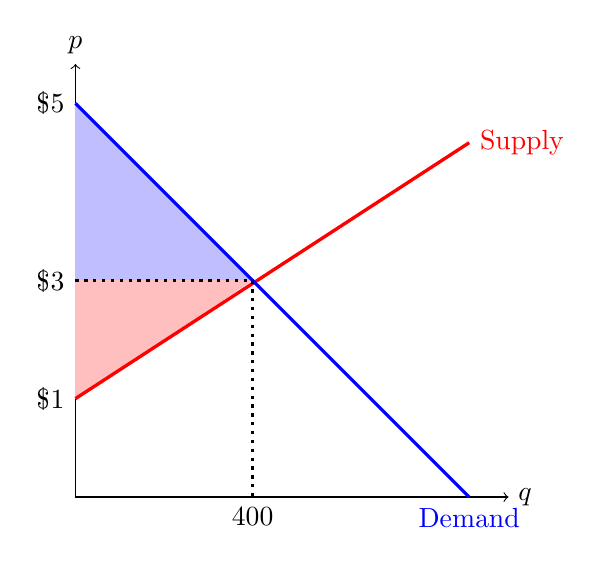
\begin{tikzpicture}[scale=.5]
		\draw[->] (0,0) -- (11,0) coordinate (x axis) node[right]{$q$};
 		\draw[->] (0,0) -- (0,11) coordinate (y axis) node[above]{$p$};	
      \draw[blue!25, fill=blue!25] (0,10)--(0,5.5)--(4.5,5.5);
      \draw[red!25, fill=red!25] (0,2.5)--(0,5.5)--(4.5,5.5);
		\draw[very thick,red] (0,2.5)node[left]{\textcolor{black}{\$1}}--(10,9)node[right]{Supply};
		\draw[very thick, blue] (0,10)node[left]{\textcolor{black}{\$5}}--(10,0)node[below]{Demand};
		\draw[very thick, dotted] (0,5.5)node[left]{\$3}--(4.5,5.5)--(4.5,0)node[below]{400};
 	\end{tikzpicture}
	\end{center}
\end{solution}

\question Calculate the price elasticty of demand and price elasticity of supply (in equilibrium).

\begin{solution}

First, demand:

$$\begin{aligned}
E&=\frac{1}{slope}\times \frac{p}{q}\\
E&=\frac{1}{(-0.005)} \times \frac{3}{400}\\
E&=-200 \times 0.0075\\
E&=-1.5\\
\end{aligned}$$

Demand is relatively elastic. For every 1\% increase (decrease) in price, consumers will buy 1.5\% less (more).

Next, supply:

$$\begin{aligned}
E&=\frac{1}{slope}\times \frac{p}{q}\\
E&=\frac{1}{(0.005)} \times \frac{3}{400}\\
E&=200 \times 0.0075\\
E&=1.5\\
\end{aligned}$$

Supply is relatively elastic. For every 1\% increase (decrease) in price, producers will well 1.5\% more (less).

Notice that demand and supply have the *same* price elasticity in equilibrium (at least in terms of magnitude, for demand it will always be negative)! The price and quantity is the same for both curves (by definition, that's equilibrium), but in this case the slopes are the same - so the elasticities will be the same. This shows you slope has a strong effect on elasticity.

\end{solution}
	
\question Calculate the consumer surplus and producer surplus, and shade each on the graph.

\begin{solution}

Consumer surplus is a triangle (shaded in blue) between the demand curve (most consumers are willing to pay) and the market price (what they actually pay). The area of the triangle is:

$$\begin{aligned}
CS &=\frac{1}{2}bh\\
CS &=\frac{1}{2}(400-0)(\$5-\$3)\\
CS &=\frac{1}{2}(400)(2)\\
CS &=\frac{1}{2}800\\
CS &=400\\
\end{aligned}$$

Producer surplus is a triangle (shaded in red) between the market price (what sellers actually recieve) and the supply curve (the lowest they would be willing to recieve). The area of the triangle is:

$$\begin{aligned}
PS &=\frac{1}{2}bh\\
PS &=\frac{1}{2}(400-0)(\$3-\$1)\\
PS &=\frac{1}{2}(400)(2)\\
PS &=\frac{1}{2}800\\
PS &=400\\
\end{aligned}$$

Both consumer and producer surplus are calculated with the same base (market equilibrium quantity), and the height of each is the difference between the market price and that curve's choke price. A curve with a choke price further away from the market price (willing to pay/accept much more/less) will have a steeper slope, a smaller elasticity in equilibrium, and therefore generate less surplus.

\end{solution}

\question Who gets greater surplus, consumers or producers, and why?

\begin{solution}

In this case, because both supply and demand have the same elasticity in equilibrium, they earn the same amount of surplus.

\end{solution}

\end{questions}

\end{document}